\documentclass[handouts]{beamer}
\usepackage[orientation=portrait,size=a4, scale=2]{beamerposter}

\input preamble.tex

\title{Ostrovní biogeografie}
\usefonttheme{serif}

\begin{document}

\begin{frame}

  \begin{center}
    \Large Ostrovní biogeografie
  \end{center}
  
  Teorii ostrovní biogegrafie vytvořili R. H. Mac Arthur a
  E. O. Wilson pro vysvětlení odlišné dynamiky populací na
  ostrovech. Jejich teorie byla později rozšířena na obecné lokality
  oddělené od okolí prostředím jiného typu a má tak smysl i pro jiné ekosystémy, než ostrovy v zeměpisném slova smyslu.

  \medskip
  Uvažujme ostrov, na který mohou z pevniny migrovat nové druhy, které
  na ostrově dosud nežijí.

% \section{Předpoklady}

  \begin{columns}
    \begin{column}[t]{0.48\hsize}
      \begin{block}{Rychlost kolonizace}
\begin{itemize}
\item Počet druhů, které v čase
$t$ proniknou na ostrov a úspěšně se zde zabydlí, roste s počtem
imigrantů  a klesá s počtem druhů, které na ostrově  již žijí (komplexnější společenstva organismů jsou stabilnější a lépe
odolávají invazi nových druhů).
\item  Počet imigrantů klesá s rostoucí
vzdáleností ostrova od pevniny.
\item  Uvedené předpoklady splňuje funkce
$$
 \frac b{D(N+\beta)},
$$
kde $N$ je počet druhů na ostrově v čase $t$, $D$ je vzdálenost ostrova od
pevniny, $\beta$ je nezáporná a  $b$ kladná konstanta. 
\end{itemize}
\end{block}
\end{column}
\begin{column}[t]{0.48\hsize}
  \begin{block}{Rychlost vymírání  druhů}

\begin{itemize}
\item Rychlost vymírání  druhů, které v minulosti již úspěšně
kolonizovaly ostrov, ale neobstály v~ konkurenci pozdějších kolonizátorů,
roste s~ klesající rozlohou ostrova a s rostoucím počtem druhů na
ostrově (ostrov menší rozlohy má menší nosnou
kapacitu).
\item Rychlost vymírání druhů je možné modelovat funkcí
$$
 a\frac {N^k}S,
$$
kde $S$ je rozloha ostrova a $a$ a $k$ jsou kladné konstanty.
\end{itemize}
\end{block}
\end{column}
\end{columns}

\bigskip
\subsection{Model}

Počet druhů na ostrově rozlohy $S$ ve
vzdálenosti $D$ od pevniny vyhovuje diferenciální rovnici
$$
  \frac{\mathrm dN}{\mathrm dt}= \frac b{D(N+\beta)}-a\frac {N^k}S.
$$
Předpokládáme-li, že na počátku byl ostrov neosídlený, připojíme
podmínku $N(0)=0$.

\subsection{Výstupy modelu}


\begin{minipage}[t]{0.5\linewidth}
  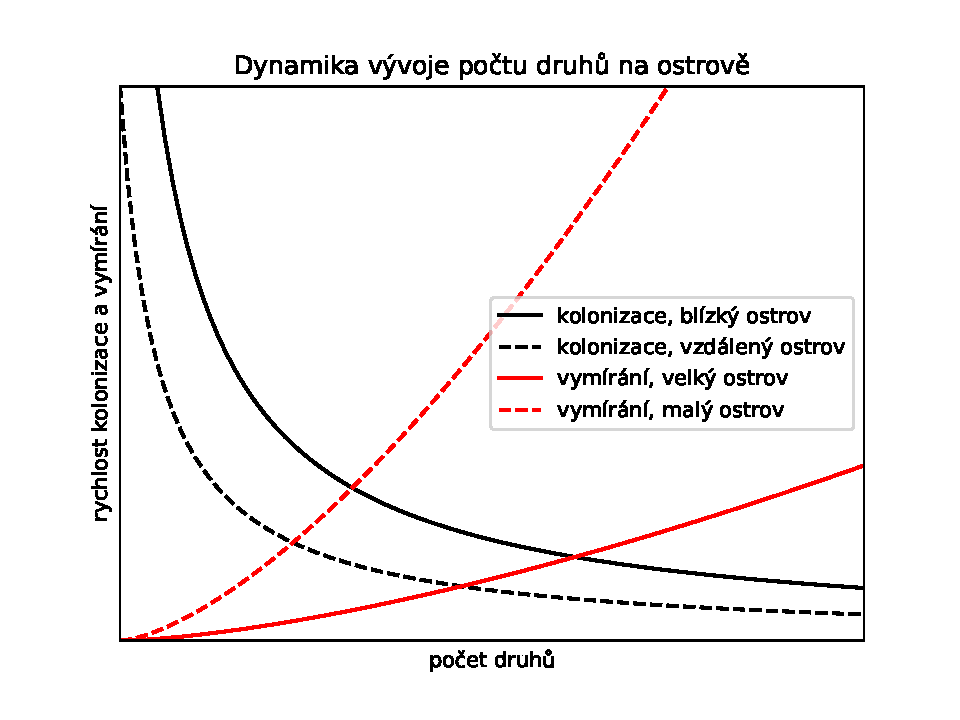
\includegraphics[width=\linewidth]{ostrov1.pdf}
\end{minipage}\begin{minipage}[t]{0.5\linewidth}
  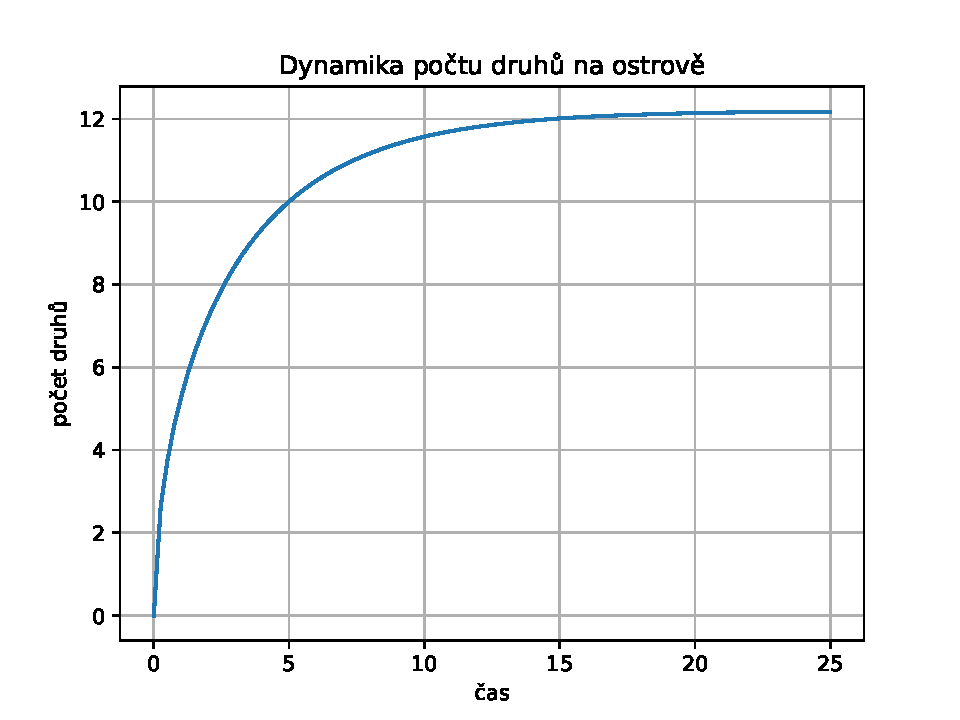
\includegraphics[width=\linewidth]{ostrov2.pdf}
\end{minipage}

Model vysvětluje, proč souvisí velikost 
lokality s počtem druhů, které trvale obývají danou lokalitu.
Předpoklady a~závěry teorie jsou ověřeny 
pozorováními i cílenými experimenty.

\end{frame}
\end{document}


%%% Local Variables: 
%%% TeX-command-extra-options: "-shell-escape"
%%% TeX-engine: xetex
%%% End:
